In recent years, machine learning (ML) has become a powerful tool if the field of HEP.

\chapter{Deep Learning Basics}

Deep learning is the subset of machine learning that focuses on the development and training of artificial neural networks.
These neural networks take the form of a series of composable, parameterized, and differentiable transformations that map input data to output data.
Training or optimization of the network is done by modifying the parameters of each transformation.
This is typically performed using gradient-based algorithms to minimize a loss metric evaluated over a dataset called the training set.
The exact form of how the loss is calculated differentiates the various types of learning, such as supervised, unsupervised, reinforcement, self-supervised, etc\footnote{There is often overlap between these categories}.

Initially, artificial neural networks were inspired by the structure of the brain, with many layers of interconnected artificial neurons processing information and sending signals to each other.
While individual neurons are simple, the emergent behaviour of the network can be complex.
As the field has evolved, the initial biological inspiration of neural networks has given way to more abstract, mathematical descriptions.
Today, network design today is driven by inductive biases, computational efficiency, observations in training dynamics, and (above all) empirical results.
From this more practical perspective, an artificial neural network is long computational graph composed of differentiable operations arranged in layers that transform between collections of real-valued tensors.
The ``depth'' of a deep learning model refers to the number of layers used in the network.

The primary distinction between deep learning and other parameterized curve fitting methods is a matter of scale.
Modern networks now contain billions of parameters, requiring large datasets, specialized hardware, and sophisticated optimization algorithms to train effectively.
As the networks have grown in size and complexity, model interpretability has become a significant challenge and an active area of research.

The above definition is intentionally broad, as it encompasses an entire field of research that has grown rapidly in the last decade.
More detailed descriptions will come by way of examples in the following sections.

\section{Supervised Learning}

Supervised Learning is often introduced first in a pedagogical setting, as it is the simplest and most intuitive form of machine learning. While it is not limited to deep learning, it is introduced here within the context of DL as it is arguably the most common form of training for deep models. Indeed, many other training frameworks in deep learning, such as reinforcement learning and unsupervised learning, can be reframed as supervised problems.

In supervised learning, a single data sample is a coupling of two variables, $s = (x, y)$, where $s \sim p(X, Y)$ is drawn from unknown joint distribution.
Here $X$ is a given observable and $Y$ is the target variable.
The goal of supervised learning is to produce a discriminative model which approximates the conditional probability distribution of the target given an observation $f(x) \approx p(Y|X=x)$.
Discriminative models which permit sampling from this distribution can also be considered generative models, which are covered in \Cref{sec:generative}.
Alternatively, discriminative models can be non-probabilistic, where they simply attempt to create a mapping from inputs to outputs, $f: X \mapsto Y$.

Supervised learning typically requires a training set $\mathcal{D}$ containing of $N$ observations and their paired targets $\mathcal{D} = \{(x_i, y_i)\}_{i=1}^N$.
These samples are usually assumed to be independent and identically distributed (i.i.d.) from the joint distribution $p(X, Y)$\footnote{Non i.i.d. data can sometimes be used by incorporating the appropriate weights during training}.
A supervised learning algorithm $f$, probabilistic or not, is selected out of some hypothesis space $\mathcal{H}$ to minimize some cost function $L(Y \times Y) \mapsto \mathbb{R}$, which is typically a measure of empirical risk over the training set.
\begin{equation}
    f = \argmin_{f \in \mathcal{H}} \frac{1}{N} \sum_{i=1}^N \mathcal{L}(\hat{y}_i = f(x_i), y_i).
\end{equation}

For now, we make no assumptions about the structure of the input or output samples except that they can be represented as tensors, or collections of tensors, of real numbers.
Common types of supervised algorithms $f$ including support vector machines, decision trees, and neural networks.
For a neural network $f_{\theta}$, the hypothesis space $\mathcal{H}$ is the set of all possible network architectures and network parameter values $\theta$.

\section{The Multi-Layer Perceptron}

The Multi-Layer Perceptron (MLP) is the simplest form of a deep neural network.
It is also referred to as a dense network, fully connected network, or sometimes confusingly as a feed-forward neural network (which is usually used to describe any network without loops in the computational graph).
In an MLP, there is a single input and output, both of which are rank-1 tensors but can have differing numbers of features.
A minimal working example of an MLP is a series of affine transformations\footnote{Often called a linear layer, but the operation almost always includes a bias term.}, each parameterized by a weight matrix $W$ and bias vector $\mathbf{b}$, followed by a non-linear activation function $\sigma$.
The depth of the MLP is the number of intermediate representations in the computational graph between the input and output.
A minimal MLP with two hidden layers can be written as
\begin{align}
    \mathbf{a}_0 &= \mathbf{x}, \\
    \mathbf{a}_1 &= \sigma_0(W_0 \mathbf{a}_0 + \mathbf{b}_0), \\
    \mathbf{a}_2 &= \sigma_1(W_1 \mathbf{a}_1 + \mathbf{b}_1), \\
    \mathbf{a}_3 = \mathbf{\hat{y}} &= \sigma_2(W_2 \mathbf{a}_2 + \mathbf{b}_2),
\end{align}
where $\mathbf{x}$ is the input, $\mathbf{y}$ is the output, and $\mathbf{a}_i$ are the intermediate representations (or activations) of the network.
The parameters of this network are is the full set of weights and biases from each layer, $\theta = \{W_0, \mathbf{b}_0, W_1, \mathbf{b}_1, W_2, \mathbf{b}_2\}$.

Activation functions exist to introduce non-linearities in the computational graph and are applied element-wise to the tensors.
As the composition of affine transformations is itself an affine transformation, not matter the depth of the MLP, it could be reparameterized as a single affine transformation, greatly hindering its expressive power.
With induced non-linearities, MLPs can be shown to be universal function approximators, given enough hidden units and the right activation functions, and this feature is the primary reason for their success in deep learning.
Practically, the expressivity of an MLP is limited by the depth of the network and size of each intermediate representation.

The activation function in the output layer is typically chosen to match the expected range of $\mathbf{y}$.
Historically, the sigmoid function was used as the primary activation in the hidden layers, due to its analogy with biological activation.
However, it can be shown that even the simplest function that breaks linearity is sufficient for universal approximation, and the ReLU function $\sigma(x) = \max(0, x)$ has become the most popular choice for hidden layers in modern networks.
Common choices for hidden layer activations are shown in \Cref{fig:activations}.

\begin{figure}
    \centering
    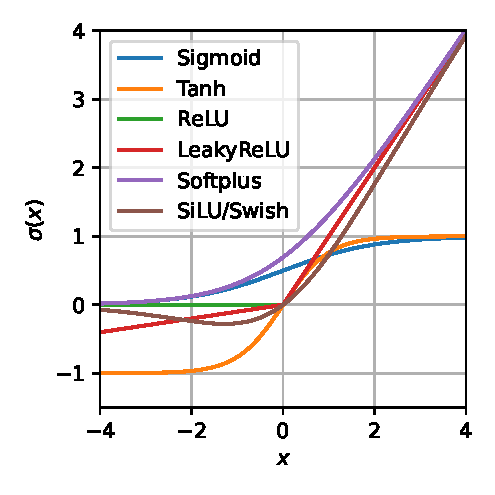
\includegraphics[width=0.4\textwidth]{Figures/transformers/activations.pdf}
    \caption{Common activation functions used in deep learning.}
    \label{fig:activations}
\end{figure}

\section{Training with Gradient Descent}

The most common method for training deep neural networks is stochastic gradient descent (SGD) or one of its many variants.
SGD is an iterative optimization algorithm that attempts to minimize a loss function by adjusting the parameters of the model in the direction of the negative gradient of the loss.
The loss function is typically a measure of the discrepancy between the model's prediction and the desired outputs, and the gradient of the loss is calculated with respect to the model parameters.

\subsection{Normalization}

\subsection{Biases}

\subsection{Regularization}

\subsection{Optimization}

\subsection{Learning Rate Scheduling}

\chapter{Graph Neural Networks}

% The following discussion on graph neural networks is primarily adapted from \textcite{GraphIntro,RelationalInductiveBiases,GraphRepresentationLearning}.

The philosophy behind graph neural networks (GNNs) is that nature is best understood when broken down into compositional elements.
Understanding these elements and the rules that define their relationships is key to understanding the system as a whole.
This reductionist approach is used by much of the scientific community, and indeed is the basis for all of particle physics.
Graphs are an example of explicitly structured data containing entities and pairwise relations between them.
Relational reasoning is the development of rules or functions that describe how the properties of entities modify the relations between them, and how the relations modify the properties of the entities.
GNNs are a class of deep learning models that operate on graph-structured data and employ relational reasoning complete tasks by directly manipulating the rules, entities, and relations of a system.

% \section{Inductive Biases For Graphs}

% The term inductive bias refers to the set of assumptions made about some task that allows a learning algorithm to favour one solution over another.
% It is the set of assumptions about the nature of the function to be learned which allows a restriction of the hypothesis space, before any data is seen.
% In practice, inductive biases typically involve the smart decisions made by a model designer which make the learning problem easier or guide the process to target a specific class of solutions.
% \todo{Cite inductive bias}

% Inductive biases do not have to be explicitly defined.
% For example, fitting a linear regression model to data assumes explicitly that the relationship between the input and output is linear.
% Doing so using the least-squares loss function implicitly assumes that the linear relationship is corrupted by Gaussian noise with constant variance.
% For deep learning, examples of inductive biases include the choice of loss function, regularization, the optimization algorithm, and even the model architecture itself.
% Weight decay can be seen as an inductive bias towards simpler models, as prioritizes solutions with small parameters.

% Ideal inductive biases should improve the performance of the model primarily by aiding the optimization process.
% However, too restrictive biases can limit model performance by excluding valid solutions.
% Inductive biases can also be understood in terms of the bias-variance trade-off, where flexibility is traded for generalization.

% \subsection{Relational Reasoning}

An example of successful relational reasoning being used in deep learning outside GNNs is in image processing tasks.
An image is typically represented as a tensor of shape $(H, W, C)$, where $H$ is the height, $W$ is the width, and $C$ is the number color channels, using the pixel values as the tensor elements.
Image processing tasks were once the domain of MLPs \citetemp{MLPforMNIST}.
This meant that the image must first be flattened to a tensor of shape $H \times W \times C$, and then passed through a series of fully connected layers, whereby every element of the input tensor is connected to every element of the output tensor.
While this leads to a flexible model, it also destroys the spatial structure of the image and no reusable relationships or rules are discovered.
Instead, we would like to use a model that preserves the structure of the data.

The building block of the convolutional neural network is a learnable convolutional kernel.
The kernel scans over the input tensor, computing the weighted sum of the elements in the kernel window.
This introduces two key relational inductive biases: locality and translation invariance.
Locality refers to the assumption that the relationship between two elements is stronger if they are close together in the input space.
Translation invariance refers to the assumption that the relationship between two elements is the same regardless of their absolute position in the input space.
Locality is enforced by using a kernel width of limited size and translation invariance is enforced by reusing the same kernel across the input space.
Each convolutional kernel defines a learned and reused rule for how elements within the structure of the input tensor are related.

This is an example of geometric deep learning, also called a relational inductive bias, whereby the known structure of the data is embedding into the architecture of the model itself, rather than being learned directly from the data.
This reduces the number of parameters required in the model, allowing for more statistically efficient learning.

\section{Defining a Graph}

A graph $\mathcal{G}$ is a data structure that consists of a set of $N$ attributed nodes $\mathcal{N} = \{\mathbf{x}_i\}_{i=1}^{N}$ interconnected by a set of $N^e$ attributed edges $\mathcal{E} = \{(\mathbf{e}_{k}, r_k, s_k)\}_{k}^{N^e}$.
Here $\mathbf{e}_{k}$ are the edge attributes, $s_k$ is the index of the sender node and $r_k$ is the index of the receiver node.
The graph is directed and self-loops are allowed.
It is also useful in many contexts to define a global attribute $\mathbf{u}$ which describes the entire graph as a whole.
A singular-graph can be represented as a tuple $\mathcal{G} = (\mathcal{N}, \mathcal{E}, \mathbf{u})$.
The structure of the graph is only defined by the interconnections between the nodes, the actual ordering of the nodes in the set is arbitrary.
Therefore, any operation on the graph should not depend on the ordering of the nodes.
Not that the adjacency matrix of the graph is not explicitly defined, but can be inferred from the elements of $\mathcal{E}$.

This representation of a graph is very general and each of the terms $\mathcal{N}$, $\mathcal{E}$, and $\mathbf{u}$ are optionally included.
For example, set data is a special case of a graph where there are no edges connecting the nodes.
Or we could allow multiple sets of edges to exist between nodes $\{\mathcal{E}^1, \mathcal{E}^2, \ldots\}$, defining a multi-graph.
An undirected graph can be represented using a fully symmetrical edge set.

Each of the edge $\mathbf{x}_i$, node $\mathbf{e}_{k}$, and global $\mathbf{u}$ properties of the graph can be encoded as any type of data, even graphs themselves.
However, in most use cases dealt with in deep learning they are real valued tensors.
It is also common for all the nodes to share the same dimensionality, and the same for the edges, imposing an equivalence between the elements of the set.
These are not strict requirements, but it simplifies the design of the model as it allows operations on the individual elements to be parameterized with standard deep learning building blocks, such as linear layers, MLPs, and CNNs.

Representing a graph in code required tuple or dictionary of real valued tensors $(\mathbf{X}, \mathbf{E}, \mathbf{U})$.
Here, $\mathbf{X} \in \mathbb{R}^{N \times d_x}$, $\mathbf{E} \in \mathbb{R}^{N \times N \times d_e}$, and $\mathbf{U} \in \mathbb{R}^{1 \times d_u}$, where $d_x$, $d_e$, and $d_u$ are the dimensionality of the node, edge, and global features respectively.
The edge matrix is typically ordered such that $\mathbf{E}_{ij}$ is the edge from node $i$ to node $j$.
To represent the existence or absence of an edge between two nodes, a binary adjacency matrix $\mathbf{A} \in \{0, 1\}^{N \times N}$ can be used where $\sum{\mathbf{A}} = N^e$.
Alternatively, one could use a sparse tensor representation, which is more memory efficient but can complicate the implementation of the model.

Almost all GNNs operate on the graph by facilitating message passing between the nodes.
In this framework the nodes send messages to their neighbours.
These messages are then aggregates and used to update the node's attributes.

\begin{figure}
    \centering
    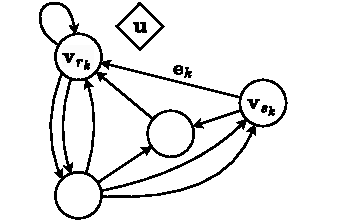
\includegraphics[width=0.5\textwidth]{Figures/transformers/graphs.pdf}
    \caption{A directed multi-graph with node, edges a global attribute $\mathbf{u}$. Highlighted is the edge $\mathbf{e}_{k}$ which connects the sender node $s_k$ to the receiver node $r_k$. Adapted from \textcite{RelationalInductiveBiases}.}
    \label{fig:graph}
\end{figure}

\section{Graph Type Data}

Graph or set representation is fairly ubiquitous in the real world and can be used for anything that can be broken down into discrete elements.
Some examples are shown in \Cref{fig:graph_examples}.
Relevant to this thesis, particle interactions may be expressed as sets, where the stable particles are the nodes.
This is natural representation for particle data, which has no inherent ordering.
Complete interactions and decay chains, like all-hadronic $ttH$ production process shown in \Cref{fig:feynman}, can be represented as a graph.
In this instance, it might be more natural to represent the virtual particles in the Feynman diagram as edges rather than the nodes.
Chemical compounds can be easily represented as graphs, where the atoms and the chemical bonds between them are the nodes and edges respectively.
\Cref{fig:chemical} shows the structure of the antibiotic rifampicin.

Text can be converted into a graph by treating words or subwords as nodes~\citetemp{AttentionIsAllYouNeed}.
Though graphs typically have no natural ordering, it can be imposed by appending the order of the element in the sequence to the attributes of each node.
The edges may also be connected such that they respect the order of the sequence, as in \Cref{fig:text}, where information can only flow forward in the sequence.
This has significant consequences for many generative modelling tasks, essentially providing a natural way to train and perform autoregressive sampling.

Even data which is not inherently graph-like can be broken down into constituent parts and interconnected as desired to form a graph.
Here, the choice of representation is crucial to the rules learned by the model.
As information can only propagate along defined edges in the graph, the existence of an edge implies a direct relationship between the sender and receiver nodes.
An image may be patched into a grid where each patch is treated as a node as shown in \Cref{fig:dog}.
Like the CNN, locality can be imposed by only connecting patches close to each other.
A patched image may not have any edge attributes at all, alternatively, translationally invariant information and could be encoded in the edge attributes, such as the vertical and horizontal distance between patches.

\begin{figure}
    \centering
    \begin{subfigure}[b]{0.45\textwidth}
        \centering
        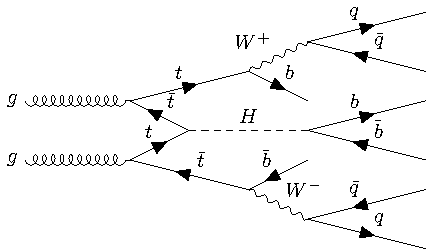
\includegraphics[width=\textwidth]{Feynman/tth.pdf}
        \caption{Particle interactions}
        \label{fig:feynman}
    \end{subfigure}
    \begin{subfigure}[b]{0.45\textwidth}
        \centering
        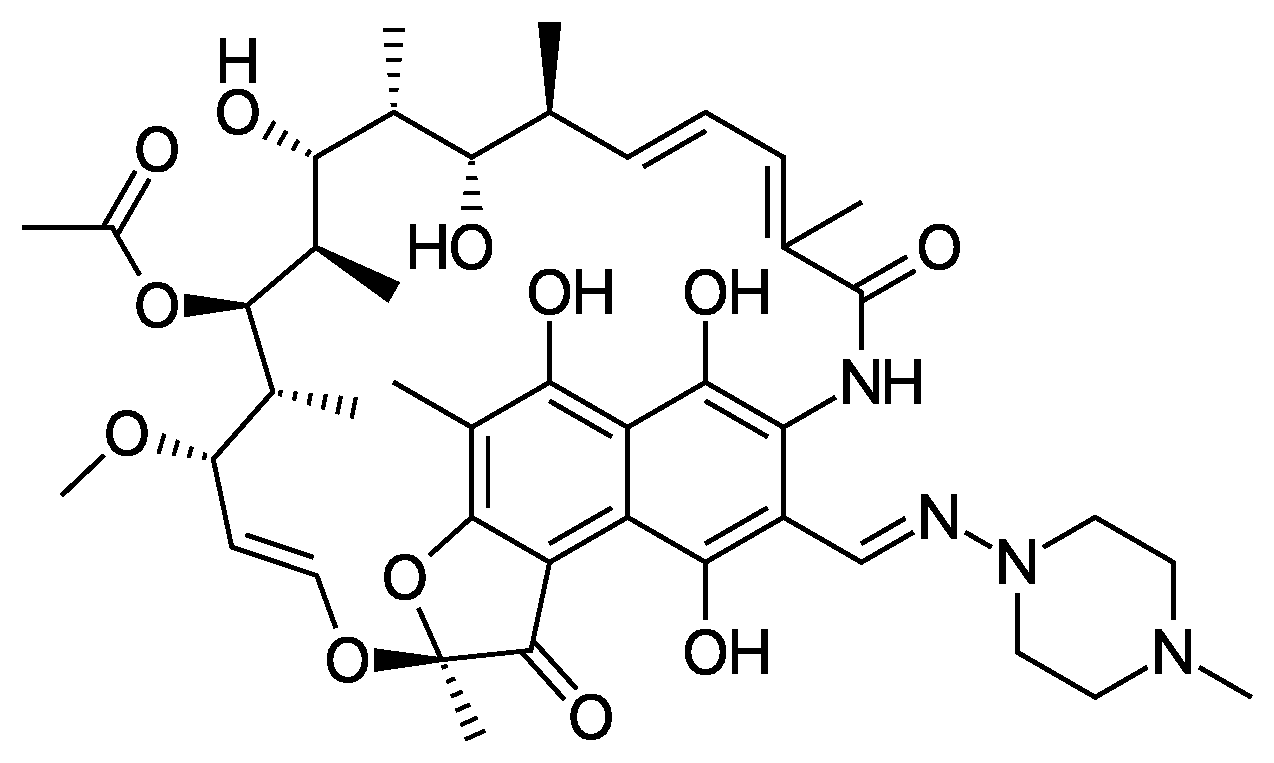
\includegraphics[width=\textwidth]{Figures/transformers/Rifampicin_structure.pdf}
        \caption{Chemical compounds}
        \label{fig:chemical}
    \end{subfigure}
    \begin{subfigure}[b]{0.45\textwidth}
        \centering
        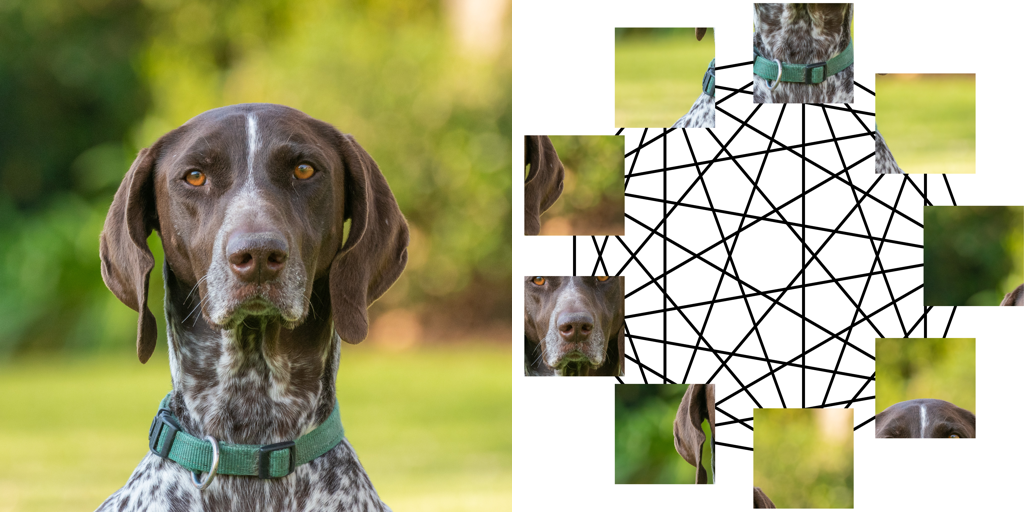
\includegraphics[width=\textwidth]{Figures/transformers/patched_image.png}
        \caption{Images (patched)}
        \label{fig:dog}
    \end{subfigure}
    \begin{subfigure}[b]{0.45\textwidth}
        \centering
        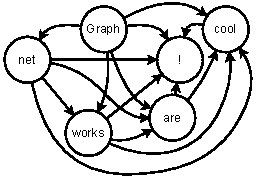
\includegraphics[width=0.8\textwidth]{Figures/transformers/text.pdf}
        \caption{Language (tokenized)}
        \label{fig:text}
    \end{subfigure}
    \caption{Examples of data that can be represented as graphs.}
    \label{fig:graph_examples}
\end{figure}

\subsection{Interconnectivity}

When constructing a graph representation of a data sample, it is crucial to consider its interconnectivity.
While locality is often a useful inductive bias, limiting the connections means that long term dependencies may get diluted.
This is because multiple rounds of message passing are required to propagate information between distant nodes as shown in \Cref{fig:neighbours}.
On each node is the number of message passing steps required to propagate information to the node $\mathbf{x}_i$.
With each round, exponentially more neighbouring nodes need to project information into a fixed-size vectors.
This phenomenon is known as the over-squashing problem, and is exacerbated by bottlenecks in the graph structure as shown in \Cref{fig:bottleneck}, where the information between nodes $\mathbf{x}_i$ and $\mathbf{x}_j$ must pass along a single edge which must also carry information from their respective neighbourhoods.

There are many proposed solutions to the over-squashing problem.
The inclusion of global features in the graph may help model long range dependencies, however the size of the global feature would need to scale with the cardinality of the set.
One solution is to increase the number of edges in the graph, allowing for more direct paths between nodes.
This procedure can be focussed around bottlenecks int he graph, identified by regions of low Forman curvature~\citetemp{Bottlenecks}.
The extreme case of this is a fully connected graph, where edges exist between all pairs of nodes in both directions.
Presenting the data as a fully connected graph allows the model to choose for itself which interactions are important, especially when equipped with an attention mechanism~\citetemp{AttentionIsAllYouNeed}.
However, this can be computationally prohibitive when the cardinality of the set is large, as the number of edges grows quadratically.
Furthermore, this would also mean sacrificing the relational inductive bias of locality.
For some cases this is still useful, for example the most successful models on images use fully connected graphs~\citetemp{VisionTransformers}.
This is because the locality in images is not always useful, for example if an object in the image is obscured and only partially visible physically separated patches.
Many models are looking to find a balance, and minimise the interconnectivity of the graph while preserving model quality~\citetemp{SparseAttention}.

Increasing the connectivity of the graph can also be applied in instances where the physical graph is not fully connected.
In the example of the chemical compound in \Cref{fig:chemical}, the edges are defined by the chemical bonds between the atoms.
However, long range dependencies may exist.
For example, the function of one part of a protein may be altered by the presence of a ligand on the other side of the molecule.
However, a fully connected graph may discount the actual chemical bonds.
One solution to this is to build a multigraph to represent close or long range interactions.
However, a large enough edge dimension, with attributes for the type of interaction, and an expressive enough update function may suffice.

This also does raise whether the computational graph and the input data structure should be tied together at all.
Recent work in vision transformers have shown that the addition of extra, fully learnable nodes to the graph can improve performance~\citetemp{Registers}.
Models which fully separate the input graph and the computational graph used for message passing include the perceiver~\citetemp{Perceiver}.

\begin{figure}
    \centering
    \begin{subfigure}[b]{0.3\textwidth}
        \centering
        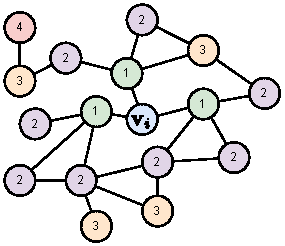
\includegraphics[width=\textwidth]{Figures/transformers/neighbours.pdf}
        \caption{}
        \label{fig:neighbours}
    \end{subfigure}
    \begin{subfigure}[b]{0.3\textwidth}
        \centering
        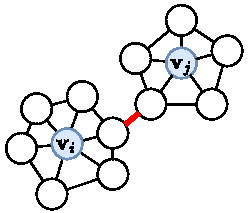
\includegraphics[width=\textwidth]{Figures/transformers/bottleneck.pdf}
        \caption{}
        \label{fig:bottleneck}
    \end{subfigure}
    \caption{\subref{fig:neighbours} The locality of information flow in a graph. \subref{fig:bottleneck} A graph with a bottleneck.}
    \label{fig:over_squashing}
\end{figure}

\subsection{Graph Tasks}

In analysing graph data within real-world contexts, there exists three primary types of predictive tasks: graph-level, node-level, and edge-level predictions.
For graph-level tasks, the aim is to predict an attribute or property that encompasses the entire system as a whole.
An example of this in the context of computer vision would be the classification of the entire image~\citetemp{VisionTransformers}.
Node-level tasks predict the properties associated with each individual node.
They are somewhat analogous to image segmentation.
Finally, there are edge-level tasks which predict  properties or even the existence of edges between the nodes.
An example of this may be predicting the type of virtual particle in a Feynman diagram, \Cref{fig:feynman}.

\section{The Graph Network Block}
\label{sec:gn_block}

The Graph Network Block (GN-Block) is a useful building block for constructing deep learning models that operate on graph-structured data.
It offers a framework that generalizes to many other existing graph-based models, such as graph convolutional networks (GCNs), graph attention networks (GATs), deep sets, and even transformers.
A GN-Block is defined as a series of operations that update the node, edge, and global attributes via facilitating the exchange and aggregation of information according to the structure of the graph.
The GN-Block does not change the cardinality of the features present, only updating their attributes,
\begin{equation}
    \text{GN}(\mathcal{N}, \mathcal{E}, \mathbf{u}) = (\mathcal{N}', \mathcal{E}', \mathbf{u}')
\end{equation}
The GN block is composed of three sub-blocks involving three update functions, $\phi^v$, $\phi^e$, and $\phi^u$, and three aggregation functions, $\rho^{e \to v}$, $\rho^{e \to u}$, and $\rho^{v \to u}$.
Given an input graph $\mathcal{G} = (\mathcal{N}, \mathcal{E}, \mathbf{u})$ the GN-Block proceeds as follows.

\begin{enumerate}
    \item \textbf{Edge Block:} The edges are updated using the current edge attributes, the attributes of the sender and receiver nodes, and the global attribute.
    \begin{equation}
        \mathbf{e}_k' = \phi^e(\mathbf{e}_k, \mathbf{x}_{s_k}, \mathbf{x}_{r_k}, \mathbf{u}).
    \end{equation}
    All edges throughout the graph are updated in this manor which can be executed in parallel.
    The updated edges can be thought of as the message being passed from the sender to the receiver.
    \item \textbf{Node Block:} Incoming edge information is aggregated for each node.
    For node with index $i$, this is represented by the set $E_i$.
    \begin{equation}
        \mathbf{\bar{e}}_i = \rho^{e \to v}(E_i) = \rho^{e \to v}\left(\{(\mathbf{e}_k', r_k, s_k) | r_k = i\}\right)
    \end{equation}
    All nodes are then updated using its current attributes, the aggregated edge information, and the global attribute.
    Updating the nodes using incoming information is called message passing.
    \begin{equation}
        \mathbf{x}_i' = \phi^v(\mathbf{\bar{e}}_i, \mathbf{x}_i, \mathbf{u}).
    \end{equation}
    \item \textbf{Global Block:} All edge information and node information across the graph is aggregated,
    \begin{alignat}{2}
        \mathbf{\bar{v}} &= \rho^{v \to u}(\mathcal{N}') &&= \rho^{v \to u}(\{\mathbf{x}_i\}_{i=1}^{N}) \\
        \mathbf{\bar{e}} &= \rho^{e \to u}(\mathcal{E}') &&= \rho^{e \to u}(\{\mathbf{e}_k'\}_{k=1}^{N^e}),
    \end{alignat}
    and used to update the global attribute,
    \begin{equation}
        \mathbf{u}' = \phi^u( \mathbf{\bar{e}}, \mathbf{\bar{v}}, \mathbf{u}).
    \end{equation}
\end{enumerate}

The GN-Block describes a basic graph to graph transformation which can be composed to form a deeper model.
To make the block learnable, each of the update or aggregation functions may be parameterized by a separate neural network.
The only requirement for any of the aggregation functions is that they are permutation invariant and may accept a variable number of arguments.
This structure also lends itself to the different types of tasks performed on graph type data.
For example, the final GN-Block in the stack may only contain an edge block for an edge-level task.

It is important to investigate exactly what inductive biases are being imposed by the GN-Block.
First, it is clear that the updates to the graph do not depend on the order of the nodes.
Formally, the node and edge updates $(\mathcal{N}, \mathcal{E}) \rightarrow (\mathcal{N}', \mathcal{E}')$ are permutation equivariant to the node set, and the global update $U \rightarrow U'$ is permutation invariant.
The GN-Block applies the same update and aggregation functions to all nodes and edges in the graph.
This reflects the relational inductive bias which seeks to learn general rules that apply to all entities in the system while also adhering to the equivalence of the elements within the set.
Furthermore, as the GN-Block only prescribes the rules for how the features of a graph are updated, it is agnostic to the structure and size of the input graph.
This allows the same model to be applied to input sets with varying cardinality.
This is a crucial feature for many applications, such as particle physics, where the number of particles in an event can vary.
Finally, information flow between elements of the set can follow two paths.
Either, the information propagates along the edges of the graph, enforcing locality, or it is aggregated into the global attribute, then redistributed to the nodes.
This allows for the model to learn both local and long-range interactions.

\section{Different Graph Networks}

A GNN is a general framework for constructing deep learning models that operate on graph-structured data.
Almost all GNNs facilitate message passing and layers within the network can be thought of as some specialization of the GN-Block, depending on the forms of the $\phi$ and $\rho$ functions, and the existence of edge, node, and global features.
The specifics of these functions mean that there are many GNN variants.

A full GN-Block is shown in \Cref{fig:full_gn_block}.
A basic implementation, where all graph attributes are tensors, can be done using MLPs for each of the update functions, and summation for the aggregation functions.
This creates the following update equations,
\newcommand{\tall}{\vphantom{\sum_{k: r_k = i}}}
\begin{equation} \label{eq:gn_update}
    \begin{aligned}
        \tall \mathbf{e}_k' &= \text{MLP}_e([\mathbf{e}_k, \mathbf{x}_{s_k}, \mathbf{x}_{r_k}, \mathbf{u}]) &&\rightarrow \text{update edge features}, \\
        \tall \mathbf{\bar{e}}_i &= \sum_{k: r_k = i} \mathbf{e}_k' &&\rightarrow \text{aggregate incoming information per node}, \\
        \tall \mathbf{x}_i' &= \text{MLP}_v([\mathbf{\bar{e}}_i, \mathbf{x}_i, \mathbf{u}]) &&\rightarrow \text{update node features}, \\
        \tall \mathbf{\bar{e}} &= \sum_{k} \mathbf{e}_k', \quad \mathbf{\bar{v}} = \sum_{i} \mathbf{x}_i' &&\rightarrow \text{aggregate features across the graph}, \\
        \tall \mathbf{u}' &= \text{MLP}_u([\mathbf{\bar{e}}, \mathbf{\bar{v}}, \mathbf{u}]) &&\rightarrow \text{update global features},
    \end{aligned}
\end{equation}

where the square brackets denote tensor concatenation.
This provides a simple model that can be trained end-to-end using gradient descent.
Other GNN layers can be framed similarly.
Even the deep set, which has no pairwise interactions between the nodes can be seen as a reduced form of a GN-Block, as shown in \Cref{fig:deep_set}.
Here the operations are simply,
\begin{align}
    \mathbf{x}_i' &= \text{MLP}_v\left(\left[\mathbf{x}_i, \mathbf{u}\right]\right),\\
    \mathbf{u}' &= \text{MLP}_u\left(\left[\sum_{i} \mathbf{x}_i', \mathbf{u}\right]\right).
\end{align}

GN-Blocks which preserve the existence of graph features, unlike the deep set which has no node features in the output, can be stacked together to form a deep GNN.
The depth of most GNNs is notably shallower than other deep learning models, such as CNNs which can have hundreds of layers.
One of the reasons for this is training instability and the over-smoothing problem.
Over-smoothing refers to the phenomenon where the nodes in the graph become homogenous, containing the same information, after many rounds of message passing.
There are many proposed solutions to this issue, such as residual connections and normalization layers.
Attention is also a viable method to combat over-smoothing.
It refers to the process of weighting the incoming messages based on some learned function of the sender and receiver nodes before aggregation.
It allows the node to ``pay more attention'' to certain neighbours.
This introduces more expressivity into the model by distinguishing the layers for deciding the content of a message and the layers for deciding its importance.

\begin{figure}
    \centering
    \begin{subfigure}[b]{0.49\textwidth}
        \centering
        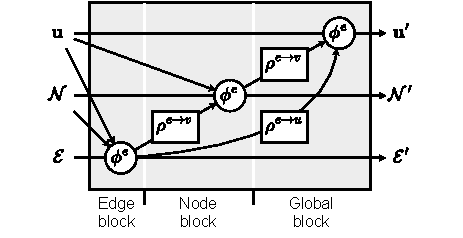
\includegraphics[width=\textwidth]{Figures/transformers/full_gn.pdf}
        \caption{Full GN Block}
        \label{fig:full_gn_block}
    \end{subfigure}
    \begin{subfigure}[b]{0.49\textwidth}
        \centering
        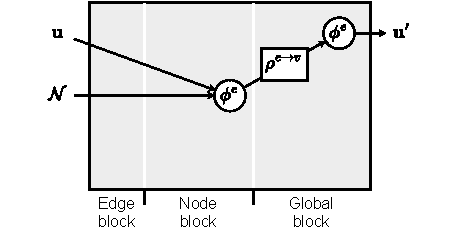
\includegraphics[width=\textwidth]{Figures/transformers/deepset.pdf}
        \caption{Deep Set}
        \label{fig:deep_set}
    \end{subfigure}
    \caption{Examples of different GN-Block implementations \subref{fig:full_gn_block} A full GN-Block has persistent edge and global features. \subref{fig:deep_set} A deep set only applies pooling to the node features to produce a global feature.}
\end{figure}

\section{Transformers are Graph Networks}

It is hard to overstate the impact of the transformer model~\citetemp{AttentionIsAllYouNeed} on the field of deep learning.
Originally designed for sequence-to-sequence tasks, transformers grew to dominate all NLP benchmarks.
They marked such a significant improvement that research in other sequence-based models, such as RNNs, almost ceased entirely.
In 2019, Google announced that they were using the transformer based BERT model~\citetemp{BERT} to power their search engine~\citetemp{GoogleBERT}.
They would also switch to using transformers for their translation service~\citetemp{GoogleTranslate}.
Starting in 2018, OpenAI began releasing the GPT~\citetemp{GPT} series of transformer models, arguably triggering a boom around large language models that continues to this day.
In 2020, transformers were adapted to work on image data~\citetemp{VisionTransformers} and have since become the state-of-the-art model for most computer vision tasks, a task that was previously dominated by CNNs, as shown in \Cref{fig:benchmarks}.
Even image generation tasks which one used UNets are now being performed by transformers~\citetemp{DIT, SD3}.
Key to the transformer success is how simple they are to implement and how well the performance seems to scale with the size of the model.
Transformers have become so ubiquitous that they are now considered the default choice for many deep learning tasks, regardless of the data type.

At its core, the vanilla transformer encoder is simply another form of a GNN\@.
There are many variants for the transformer model, but they all share the same basic features.
Contrary to popular belief, these models do not natively run on sequences but on sets, and must be adapted to work on data with an inherent order.
We will focus on two main types of transformers, the transformer encoder and the transformer decoder.
Specifically, the transformer encoder can be seen as a non-local neural network (NLNN)~\citetemp{NLNN} as shown in \Cref{fig:transformer}.
This function operates on a pure set, with no persistent edge or global features.
It involves and message passing step, done using multi-headed attention, followed by a node update step using an MLP.
They also employ residual connections and many forms of normalization to stabilize training and prevent over-smoothing.

The jargon of transformers differs slightly from that of GNNs.
Graphs and sets contain nodes, which are called tokens in many papers on transformers.
The term attention is also used more broadly in transformers, not just referring to the means of weighting an aggregation, it is sometimes used to refer to the entire message passing step.
Furthermore, saying that a node attends to another is equivalent to saying that the node receives a message from the other.
People
The adjacency matrix in a graph is also called the attention mask in a transformer.

\begin{figure}
    \centering
    \begin{subfigure}[b]{0.49\textwidth}
        \centering
        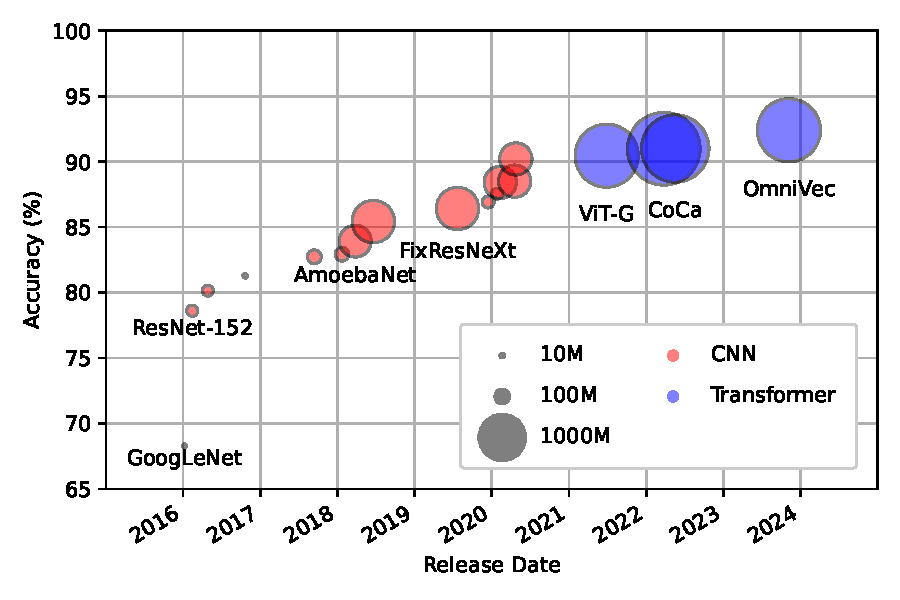
\includegraphics[width=\textwidth]{Figures/transformers/imagenet.pdf}
        \caption{}
        \label{fig:imagenet}
    \end{subfigure}
    \hfill
    \begin{subfigure}[b]{0.49\textwidth}
        \centering
        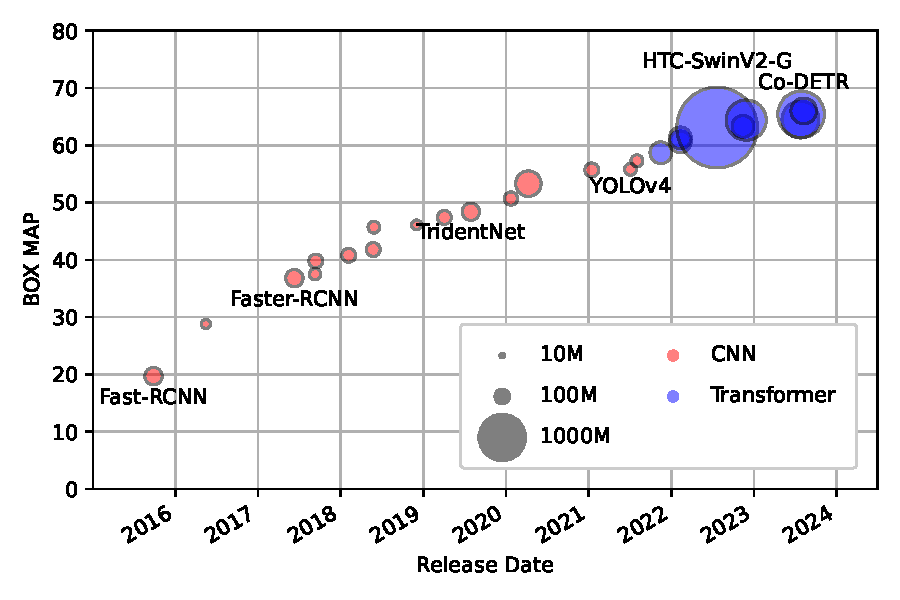
\includegraphics[width=\textwidth]{Figures/transformers/coco.pdf}
        \caption{}
        \label{fig:coco}
    \end{subfigure}
    \caption{Evolution of the state-of-the-art models in two common computer vision benchmarks~\cite{paperswithcode}. The size of the markers corresponds to the number of trainable parameters in the model. \subref{fig:imagenet} Accuracy on the ImageNet classification benchmark, \subref{fig:coco} Bounding box mean average precision (BOX MAP) the COCO object detection benchmark.}
    \label{fig:benchmarks}
\end{figure}

\begin{figure}
    \centering
    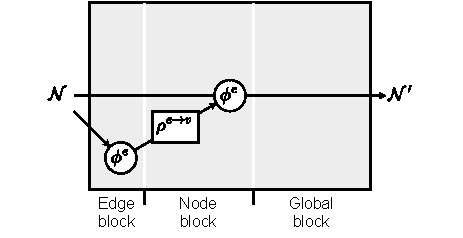
\includegraphics[width=0.49\textwidth]{Figures/transformers/nonlocal.pdf}
    \caption{NLNN / Transformer Encoder}
    \label{fig:transformer}
\end{figure}

\subsection{Attention is Message Passing}
\label{sec:attention}

There are hundreds of ways to parameterize the message passing step in a GNN, and the one used in the transformer is the scaled dot-product attention (SDPA).

In SDPA, the message passed between nodes is a linear projection of the sender node attributes.
This means that each node sends out the same message to all of its neighbours.
This sent information is referred to as the value of the node, where is a learnable weight matrix.
The attention weight is based on a dot product between separate projections of the sender and receiver nodes, called the key and query respectively.
A softmax function is applied to the attention weights to turn the aggregation operation into a weighted mean of the incoming messages.
To prevent the gradients from exploding, the attention logits are scaled by the square root of the dimensionality of the key and value tensors $d_k$.

In the framing of the GN-Block, self-attention has the edge update is factorized into a tuple containing a scalar expressing the message weight $a_k'(\mathbf{x}_{s_k}, \mathbf{x}_{r_k})$ and a vector function for calculating the message content $\mathbf{v}_k'(\mathbf{x}_{s_k})$.
Only $\alpha^e$ depends on the pairwise interaction of both the sender and receiver nodes.
The pooling operation $\rho^{e \to v}$ normalizes over the receiver weights before aggregating the messages.
The block can be written as,
\begin{equation}
    \begin{aligned}
        \mathbf{e}_k' &= \phi^e(\mathbf{e}_k, \mathbf{x}_{s_k}, \mathbf{x}_{r_k}, \mathbf{u}) \\
        &= ( a_k', \mathbf{v}_k' ) \\
        &= \left( \exp \left( \frac{1}{d_k} \mathbf{W}^q \mathbf{x}_{s_k} \cdot \mathbf{W}^k \mathbf{x}_{r_k} \right), \mathbf{W}^v \mathbf{x}_{s_k} \right), \\
        \mathbf{\bar{e}}_i &= \rho^{e \to v}(E_i) \\
       &= \frac{\sum_{k: r_k = i} a_k' \mathbf{v}_k'}{\sum_{k: r_k = i} a_k'}.
    \end{aligned}
\end{equation}
for learnable weight matrices $\mathbf{W}^k \in \mathbb{R}^{d \times d_k}$, $\mathbf{W}^q \times \mathbb{R}^{d \times d_k}$, and $\mathbf{W}^v \in \mathbb{R}^{d \times d_v}$.

This operation can be done efficiently for all nodes in parallel using basic matrix operations.
Furthermore, it allows us to extend to two forms, self-attention and cross-attention, both expressible by the following equation,
\begin{equation}
    \label{eq:attention}
    \text{Attention}(\mathbf{X_r}, \mathbf{X_s}) = \text{softmax}\left(\frac{\mathbf{X_s} \mathbf{W}^q (\mathbf{X_r} \mathbf{W}^k)^T}{d_k} + \mathbf{B}\right) \mathbf{X_s} \mathbf{W}^v.
\end{equation}
In this expression we distinguish between the tensor representing the sender nodes $\mathbf{X_s} \in \mathbb{R}^{N_s \times d}$ and the receiver nodes $\mathbf{X_r} \in \mathbb{R}^{N_r \times d}$.
Self-attention is where the sender and receiver set are the same $\mathbf{X_s} = \mathbf{X_r}$.
This is the standard message passing operation between nodes in a graph.
Cross-attention is where the sender set and receiver set is different $\mathbf{X_s} \neq \mathbf{X_r}$.
This operation is permutation invariant with respect to $\mathbf{X_s}$ and equivariant with respect to $\mathbf{X_r}$.
As shown by \Cref{fig:bipartite}, one can interpret this as the construction of a one-way bipartite graph between two sets, where all nodes in the sender set send messages to all nodes in the receiver set.
The output of the operation would therefore be the updates to the receiver nodes.
Note that the cardinality of the sender and receiver sets do not need to be the same.
Cross-attention is a powerful tool to condition one set on another and is used in many sequence to sequence tasks, from translation to image captioning and text to image generation.
Finally, the bias term $\mathbf{B}$ is a matrix of shape $(N_r, N_s)$ which is broadcasted to the shape of the attention logits.
This can be used to focus or ignore certain pairs of nodes.

\begin{figure}
    \centering
    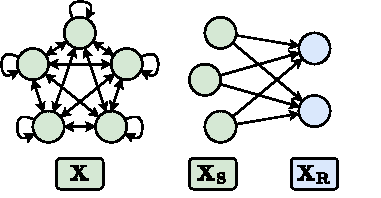
\includegraphics[width=0.5\textwidth]{Figures/transformers/bipartite.pdf}
    \caption{(left) Self-attention is standard message passing between all nodes in a graph. (right) Cross-attention creates a one-way bipartite graph between two sets of nodes.}
    \label{fig:bipartite}
\end{figure}

The final major feature of a transformer's message passing step is multi-headed attention (MHA), shown in \Cref{fig:mha}.
This is where the operation is performed multiple time in parallel with different matrices $\mathbf{W}^q$, $\mathbf{W}^k$, $\mathbf{W}^v$, and $\mathbf{B}$.
The output of each head is concatenated and then mixed using a final linear layer.
\begin{equation}
    \begin{aligned}
    & \text{Head}_1 = \text{Attention}(\mathbf{X_r}, \mathbf{X_s}), \\
    & \ldots, \\
    & \text{Head}_H = \text{Attention}(\mathbf{X_r}, \mathbf{X_s}), \\
    \vphantom{x} \\
    & \text{MHA}(\mathbf{X_r}, \mathbf{X_s}) = \text{Concat}(\text{Head}_1, \ldots, \text{Head}_H) \mathbf{W}^o,
    \end{aligned}
\end{equation}
By performing the operation many times like this, many types of messages are passed between the nodes.
One can also think of this as constructing a multi-graph with different edge types each facilitated by a different head.
Both self and cross attention can be multi-headed where multi-headed self-attention (MHSA) is defined as $\text{MHSA}(\mathbf{X}) = \text{MHA}(\mathbf{X}, \mathbf{X})$.

\begin{figure}
    \centering
    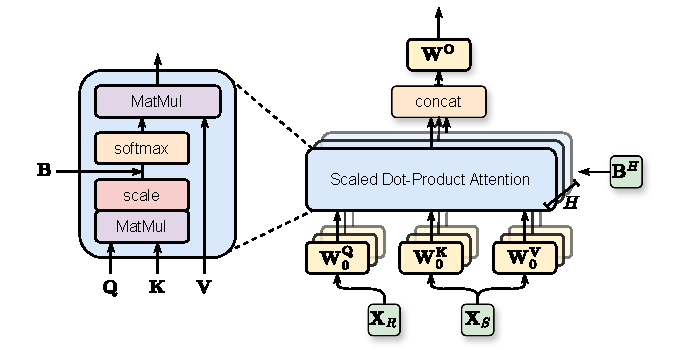
\includegraphics[width=0.5\textwidth]{Figures/transformers/mha.pdf}
    \caption{Multi-headed attention can be thought of as constructing a multi-graph with different edge types.}
    \label{fig:mha}
\end{figure}

While it is not a mathematical requirement, in practice the MHA operation is typically non-resizing, the output matches the input tensor $\mathbf{X_r}$ in shape $(N_r, d_x)$.
The SPDA mechanism requires the query and key dimensions to be the same, but in most implementations the value dimension is also matches.
This means that a single MHA function is parametrized by four weight matrices each with shape $(d_x, d_x)$.
Thus the only hyperparameter for the block is the number of heads $H$, which is required to divide into the node dimension.
One can change value and query projections from linear to affine transformations by including bias terms to increase the expressivity of the model, but the bias of the key operation is completly redundant~\citetemp{RoleOfBiases}.

One of the other keys to the transformer's success is the ease of implementation.
Many of the GNN variants require custom libraries and are difficult to implement from scratch.
However MHA can be implemented in PyTorch using standard linear algebra operations as shown in \Cref{code:attention}.
All heads are computed in parallel using smart reshaping of the tensors.
This is quite significant, as it eases the process of designing, building, testing, and exporting models.
\begin{figure}
    \centering
    \scriptsize
    \begin{minted}{python}
    class Attention(nn.Module):
        def __init__(self, dim: int, num_heads: int):
            super().__init__()
            self.NH = num_heads
            self.HD = dim // num_heads
            self.scale = self.HD**-0.5
            self.wk = nn.Linear(dim, dim)
            self.wq = nn.Linear(dim, dim)
            self.wv = nn.Linear(dim, dim)
            self.wo = nn.Linear(dim, dim)

        def forward(self, xr: T.Tensor, xs: T.Tensor, bias: T.Tensor | int = 0) -> T.Tensor:
            q, k, v = self.wq(xs), self.wk(xr), self.wv(xs)              # project
            shape = (xr.shape[0], -1, self.NH, self.HD)                  # split heads
            q, k, v = (t.view(shape).transpose(1, 2) for t in (q, k, v))
            attn = (q @ k.transpose(-2, -1))                             # attention weight
            attn = (attn * self.scale + bias).softmax(dim=-1)
            x = attn @ v                                                 # aggregate
            x = x.transpose(1, 2).reshape(B, N, D)                       # mix heads
            return self.wo(x)
    \end{minted}
    \caption{A simple implementation of a multi-headed attention block in PyTorch.}
    \label{code:attention}
\end{figure}

\subsubsection{Efficiency of Scaled Dot-Product Attention}

SDPA is arguably the most efficient form of expressive message passing suitable for fully connected graphs.
To show this it is worth starting from the simplest GNN variant, the graph convolutional network (GCN)~\citetemp{GCN}, and seeing why it fails.
The GCN is a form of NLNN where each node sends the exact same message to all other nodes; a simple linear transformation of its own attributes.
The features are then replaced by a sum over incoming information.
A GCN layer can be written as (without normalization factors),
\begin{equation}
    \begin{aligned}
    \mathbf{e}_k' &= \mathbf{W} \mathbf{x}_{s_k}, \\
    \mathbf{x}_i' &= \sum_{k:r_k=i} \mathbf{e}_k',
    \end{aligned}
\end{equation}
for a single learnable weight matrix $\mathbf{W}$.
Lets consider the shapes of the tensors in this operation.
If we represent the set of nodes as a real valued tensor, it will have shape $(N, D)$, where $D$ is the dimensionality of the attributes.
The operation $\mathbf{W}: (N, D) \rightarrow (N, D)$ is efficient, but why this fails to form good representations is clear if we consider the case where the graph is fully connected and the number of edges is $N^2$.
Since all nodes have access to all others, including themselves, however after a single update step every node in the set will contain the same information, taking the over-smoothing problem to the extreme.

To prevent this from happening, each message must be unique for each possible pairing of nodes.
So the issue becomes; what is the most efficient way to parameterize a message such that the output of the message passing must be a tensor of shape $(N, N, D)$?
Here, the first dimension is over the sender nodes and the second dimension is the receiver nodes.
The pooling operation would act over the first dimension to produce a tensor of shape $(N, D)$.
\begin{align}
    \text{??}: (N, D) & \rightarrow (N, N, D) \\
    \text{pool}: (N, N, D) & \rightarrow (N, D)
\end{align}
The GN-Block offers a way to perform this by making the message depend on a concatenation of the sender and receiver attributes.
This concatenation must be done for all possible pairings before passing this tensor through an MLP.
The operations and dimensions of the tensors of such a block are,
\begin{align}
    \text{concatenate}: (N, D) & \rightarrow (N, N, 2D) \\
    \mathbf{MLP}: (N, N, 2D) & \rightarrow (N, N, D) \\
    \text{sum}: (N, N, D) & \rightarrow (N, D)
\end{align}
Even if we were to use a single linear layer rather than an MLP, having both the input and output tensor be $O(N^2)$ is computationally expensive.

One way to mitigate this is to factorize the message into two learnable components, the content and the weight.
Only one of these needs to be unique for each pairing and since the weight is a scalar and the content is a vector, it is much more efficient to allow the content to be degenerate.
This is exactly the approach of GATs~\citetemp{GAT}, which perform the update,
\begin{align}
    \mathbf{W_1}&: (N, D)  \rightarrow (N, D) \\
    \text{concatenate}&: (N, D)  \rightarrow (N, N, 2D) \\
    \mathbf{W_2}&: (N, N, 2D)  \rightarrow (N, N) \\
    \text{matrix multiply}&: (N, N), (N, D)  \rightarrow (N, D)
\end{align}
However, there is still the issue that this input and output of the learnable layers are $O(N^2)$.

The $(N, N)$ matrix of attention weights needs to be learnable from the original $(N, D)$ node attributes and must be allowed to be unique for each pairing.
Therefore, there must be a distinction between the sender and receiver nodes, this makes the required map $a: (N, D), (N, D) \rightarrow (N, N)$.
There are few operations that can achieve this, and none so efficient as a dot product.
Using linear projections for the initial embeddings means that the K, Q, V tensors can be computed in parallel.
\begin{align}
    \mathbf{W}: (N, D) & \rightarrow (N, 3D) \\
    \text{split}: (N, 3D) & \rightarrow (N, D), (N, D), (N, D) \\
    \text{scale-dot-softmax}: (N, D), (N, D) & \rightarrow (N, N) \\
    \text{matrix multiply}: (N, N), (N, D) & \rightarrow (N, D)
\end{align}
While the other parts of the update do require $O(N^2)$ operations, crucially the input and output of the learnable layers dependent is only $O(N)$.

The argument made here is that one will struggle to find a more simple and efficient way to parameterize the message passing step in a GNN that does not lead to over-smoothing when fully connected.
The philosophy of the transformer is similar to the philosophy of composing MLPs from linear layers, in that the composition of simple, highly parameterized functions, is what provides expressivity.
By and large the most complex component of the operation is the softmax function, but there exist algorithms to calculate this online without having to express the full attention matrix~\citetemp{FlashAttention}.
Contrary to popular claims, self-attention with these mechanisms is non $O(N^2)$ in memory complexity~\citetemp{MemoryComplexity}.
Some more recent models large models have even done away with the softmax, citing better performance beyond a certain model scale~\citetemp{Reformer, LinearAttetnion}.

\section{Transformer Variants}

There are many types of transformer variants, too much to cover in this thesis.
However, common similarities can be drawn between them.
Furthermore, many of the terminology used to describe the layers is ambiguous and overlaps.
A single transformer block has two main types of sub-blocks, the message passing layer performed with MHA, and node update layers performed using MLPs, often confusingly called simply feed-forward networks (FFNs).
These sub-blocks are combined, and repeated in various forms to create the larger transformer block.
The MHA layers are configured to be either self-attention or cross-attention as needed, and they are stacked with the FFN layers usually in series~\citetemp{AttentionIsAllYouNeed}, but sometimes in parallel~\citetemp{PALM}.
Another distinguishing feature is the use of residual connections and normalization layers to stabilize training.
But even these can be configured in many ways.
With such a large zoo of transformer variants, with empirical performance being the only guide, it often takes time for best practices to emerge.

The MLP in most transformer layers only has a single hidden layer, which expands the dimensionality of the node attributes by a multiplicative factor $M$.
The original implementation used $M=4$ and a ReLU activation function,
\begin{equation}
    \phi^v(\mathbf{x}_i) = \max\left(0, \mathbf{W}_2 \text{ReLU}(\mathbf{W}_1 \mathbf{x}_i + \mathbf{b}_1) + \mathbf{b}_2\right),
\end{equation}
though these were quickly switched to either GELU of SiLU activations~\citetemp{GELU, SiLUTransformers}.
Modern transformers also use Gated Linear Units (GLU)~\citetemp{GLU}, a network layer involving the element-wise multiplication of two linear projections, one of which is passed through an activation function.
Using a Swish/SiLU activation function seems to be the most popular choice~\citetemp{SwiGLU}, the node update using a SwiGLU layer is written as,
\begin{equation}
    \phi^v(\mathbf{x}_i) = \mathbf{W}_3(\text{Swish}(\mathbf{W}_1 \mathbf{x}_i + \mathbf{b}_1) \otimes (\mathbf{W}_2 \mathbf{x}_i + \mathbf{b}_2)) + \mathbf{b}_3.
\end{equation}
Many transformers also use the mixture-of-experts approach, where there exist many FFN layers, each with different parameters, and a gating mechanism to direct certain nodes to certain experts~\citetemp{MoE}.
It is interesting that while the attention mechinism is often hailed as the key to the transformer's sucess, the vast majority of the transformer parameters are in these node update layers.

To stabilize the training of deep models, the transformer encoder uses residual connections and normalization layers.
The residual connection is used to circumvent each sub-block, and in the original implementation used LayerNorm~\citetemp{LayerNorm} after the residual connection.
This was discovered to be over squashing the signal and most modern transformers now use PreNorm configuration where the normalization is done before each sub-block~\citetemp{PreNorm}.
Many models also use RMSNorm as a faster alternative~\citetemp{RMSNorm}.
Furthermore, extra normalization within the sub-blocks is common.
It is also common to initialize the weights of the final layers in each sub-block to zero, or include extra layers initialised close to zero, such that upon initialization the model behaves like an identity function.
This greatly helps to stabilize deeper models.

The transformer encoder (TE) is a standard GNN where the message passing step is performed using multi-headed attention.
It acts on a single set of nodes, and the output of the block is the updated node attributes.
A single TE-Block as shown in \Cref{fig:transformer} is a GN-Block with no edge or global features and the message passing step is done using MHSA.
The block update on the full tensor $\mathbf{X}$, using the PreNorm configuration is,
\begin{equation}
\begin{aligned}
    \mathbf{X} & \leftarrow \mathbf{X} + \text{MSHA}(L(\mathbf{X})), \\
    \mathbf{X} & \leftarrow \mathbf{X} + \text{FFN}(L(\mathbf{X})).
\end{aligned}
\end{equation}
A full TE is composed of many TE-Blocks stacked in series forming a permutation equivariant set to set transformation.
For many tasks, the TE is the main feature extractor.

If one wanted to condition the update of one set on another, they could include a multi-headed cross attention operation in the block.
This is the original implementation of the transformer decoder (TD)~\citetemp{AttentionIsAllYouNeed}.
The update is written as,
\begin{equation}
\begin{aligned}
    \mathbf{X}_r & \leftarrow \mathbf{X}_r + \text{MHSA}(L(\mathbf{X}_r)), \\
    \mathbf{X}_r & \leftarrow \mathbf{X}_r + \text{MHA}(L(\mathbf{X}_r), \mathbf{X}_s), \\
    \mathbf{X}_r & \leftarrow \mathbf{X}_r + \text{FFN}(L(\mathbf{X_r})).
\end{aligned}
\end{equation}
The transformer encoder and decoder are often combined to form a set to set transformation that first extracts features from the input set, and the conditions the output set on these features.
This set-to-set transformation is the basis of many generative of sequence-to-sequence models.

\subsection{Edge Attributes, Biases, and Sequences}

When one views the transformer as a simple GNN, the inclusion of edge information become natural.
For message passing on a single graph, when not represented sparsely, the edge information is stored in an $\mathbf{E} \in \mathbb{R}^{N \times N \times d_e}$ tensor.
In the self attention operation in \cref{eq:attention}, the attention matrix defined by,
\begin{equation}
    \mathbf{A} = \text{softmax}\left( \frac{\mathbf{Q} \mathbf{K}^T}{d_k} + \mathbf{B} \right),
\end{equation}
which has the shape $(N, N)$.
When extending this operation to multi-headed attention it gains an extra dimension $(N, N, H)$ matching the required shape of the edge tensor, in fact it is the only valid candidate within the entire operation.
The query and key tensors $\mathbf{Q}$ and $\mathbf{K}$ stem from projections of the input, but $\mathbf{B}$ must have shape which is at least broadcastable to $(N, N, H)$.
Thus edge information can be included in a transformer through the bias term in the attention operation.
This is used in various cases.

The most common use of the bias tensor is to set it manually to negative infinity for certain pairs of nodes and for all heads.
This forces the attention weight to be zero, after the softmax operation, killing the weight of the message entirely.
This enables the transformer to run on graphs which are not fully connected.
It is also one of the main mechanisms for adapting the transformer to work on sequences, where the nodes are presented in a specific order.
By making the bias matrix a lower triangular matrix with above diagonal entries set to negative infinity, each node can only receive messages from those preceding it.
This is also called a causal mask, and is used extensively generative models as it lends itself to autoregressive sampling.
One of the main reasons why the transformer is so successful compared to other sequence models such as an RNN is that a causal attention mask allows it to parallelize training for each element in the sequence with a single forward pass.
During generation of course the model must be run sequentially, but this is a small price to pay for the increase in training speed.
Many sequence generating models are called decoder only, however in the presented framework, these models are transformer encoders with a causal mask.

While can be shown that a causal mask is enough enable the transformer able to run on sequence data, it is often paired with positional encoding.
Absolute positional encoding (APE) adds to the node attributes knowledge of their position within the sequence.
A unique tensor $\mathbf{p}_i \in \mathbb{R}^{d_x}$ is constructed for each posible observed position $i$ and is added to the node attributes before the first transformer block, $\mathbf{x}_i \leftarrow \mathbf{x}_i + \mathbf{p}_i$.
The original transformer used fixed sinusoidal functions of different frequencies to encode the position, but more recent models allow $\mathbf{p}_i$ to be fully learnable~\citetemp{GPT}.
PE is also used for images in, often called spatial encoding, where the 2D coordinates of a patch are individually encoded and added to the patch representation.

APE is not effective for allowing the model to capture the relative position of the elements in the sequence, and for this we turn to relative positional encoding (RPE)~\citetemp{RPE}.
RPE is used to bias the attention matrix and can thus be thought of as a form of edge information.
As with all transformer features, there are many approaches to RPE.
One such method to parameterise $B$ as a Toeplitz matrix, where the elements of the matrix are learnable~\citetemp{RPE}.
ALiBi~\citetemp{ALiBi} fixes the elements of this matrix to be simply $B_{ij} = m\times(i - j)$, for a fixed per-head scalar $m$.
Rotary Positional Encoding is a form of RPE where the query and key tensors are rotated by a fixed amount before the attention operation~\citetemp{RotaryPE}.

Other than positional encoding, transformers can incorporate edge information that are not dependant on order.
The Particle Transformer (PartT)~\citetemp{PartT} uses a transformer encoder to embed a set of particles, defined by their kinematics.
For each pair of particles, specific edge features are constructed using Lund Plane variables~\citetemp{LundPlane}.
The model uses an MLP to embed these edge features into a tensor of shape $(N, N, H)$, which becomes the attention bias in each of the TE-Blocks.

\subsection{Global Attributes}

Global attributes are common features in graphs, and are often used to condition the main node update or are used as outputs of the model.
Global attributes in a GNN are often updated via pooling information across all nodes in the graph $ \mathbf{u} = \rho^{v \to u}(\mathbf{X})$.
This is done in the transformer by simply summing the node attributes.
However, keeping with the theme, the cross-attention mechanism provides a pooling operation that is more expressive, even when the cardinality of the receiving set is one.
This is often called class attention~\citetemp{GoingDeeper}, and in many vision transformer models in order to classify the image as a whole.
The class attention operation can be described as,
\begin{equation}
    \mathbf{U} \leftarrow \mathbf{U} + \text{MHA}(\mathbf{U}, \mathbf{X}),
\end{equation}
where the initial embeddings of the global attributes are learnable.
This process can also be repeated to perform multiple rounds of pooling.

An alternative method relies on the fact that since most transformers act on fully connected graphs, information is not localized.
Therefore, one can simply append a new global toke (often called a class token) to the set which is updated in the same way as the other nodes~\citetemp{VisionTransformers}.
Then to classify the set, class token is read off from the final layer of node attributes.
Recent work on vision transformers have shown that using multiple global tokens in this way, called registers~\citetemp{Registers}, can improve the performance of the model.
Registers can even be ignored from the model outputs, which means that they provide the model with a temporary memory that can be used to store global information.
This is because it was observed that the models had a tendency to overwrite patches with low local information content.




One can use global attributes or extra conditional information to augment the message passing step.
If the global attributes are



This is commonly seen in diffusion models where TE-Blocks must incoroprate time information, expressed as an encoded vector.
This can be done by concatenating the $mathbf{u}$ vector to all node attributes during the MHA step~citetemp{DiffT} or the MLP step~citetemp{PCJedi}.
However the most effective way has been to combine adaptive normalization and residual gating mechanisms~citetemp{DiT}.
Here the global attribute




\chapter{Flavour Tagging with Transformers}

\section{Datasets}

\section{Input Features}

\section{Model Design}

\section{Training}

\section{Performance}

\section{Applications}










